\documentclass[a4papaer,12pt]{article}

\usepackage[left=25mm, top=20mm, right=25mm, bottom=30mm,nohead,nofoot]{geometry}

% locale settings
\usepackage[T2A]{fontenc}
\usepackage[utf8]{inputenc}
\usepackage[english,russian]{babel}

% graphics settings
\usepackage[compatibility=false]{caption}
\usepackage{subcaption}
\usepackage{wrapfig}
\usepackage{graphics, graphicx}
\graphicspath{{./images/}}
\setcounter{tocdepth}{4}

% hyperlinks settings
\usepackage{hyperref}
\hypersetup{unicode=true}

\usepackage{amssymb,latexsym} 
\usepackage{MnSymbol}
\usepackage{mathrsfs}

\usepackage[nottoc,numbib]{tocbibind}
\usepackage{float}
\usepackage{listings}
\usepackage{multirow}
\usepackage{hhline}
\usepackage{delarray}

\usepackage{color,colortbl}

\renewcommand{\listoffigures}{\begingroup  % add number to list of graphics
\tocsection
\tocfile{\listfigurename}{lof}
\endgroup}
\renewcommand{\listoftables}{\begingroup  % add number to list of tables
\tocsection
\tocfile{\listtablename}{lot}
\endgroup}

\begin{document}
\begin{titlepage}
	\center
		Санкт-Петербургский Политехнический
		университет \\ Петра Великого\\
		Институт прикладной математики и механики
		\\ \textbf{Высшая школа прикладной математики и вычислительной физики}

	\vfill ~
	\textbf{
		\\ \large КУРСОВАЯ РАБОТА \\
        Разработка контроллера светофоров и его верификация
	}
	\\ по дисциплине
	\\ "Верификация распределённых алгоритмов и протоколов"

	\vfill ~

    \begin{flushleft}
    Выполнил: \\ студент гр.3640102/00201  \hspace{\fill} \textbf{Лансков.Н.В.} \linebreak[4]
    Преподаватель: \\ к.т.н, доцент ВШПИ ИКНТ \hspace{\fill} \textbf{Шошмина И.В} \\
    \end{flushleft}

\vfill

{\large}	Санкт-Петербург
\\ 2020
\end{titlepage}

\tableofcontents 
%\newpage
\listoffigures
\listoftables
\newpage

\section{Постановка задачи}

Дан перекрёсток с четырьмя двухсторонними направлениями движения. В каждом направлении имеются
три полосы. Точная схема перекрёстка задаётся пересечениями направлений движения, указанными 
в таблице \ref{table:1}

\textbf{Вариант: 12, 13, 15}

\begin{table}[h!]
  \centering
  \begin{tabular}{| c | c || c | c |}
    \hline
      \textbf{Вариант}  & \textbf{Пересечение}  & \textbf{Вариант}  & \textbf{Пересечение}   \\
    \hline
            1        &  WN, NS        &  9        &  SN, WE  \\
    \hline
            2        &  WN, NE        &  10        &  SN, EW  \\
    \hline
            3        &  WN, SW        &  11        &  SN, ES  \\
    \hline
            4        &  WN, EW        &  \textbf{12} & \textbf{NE, EW}  \\
    \hline
            5        &  NS, SW        &  \textbf{13} &  \textbf{NE, ES}  \\
    \hline
            6        &  NS, WE        &  14        &  SW, WE  \\
    \hline
            7        &  NS, EW        &  \textbf{15} &  \textbf{SW, ES}  \\
    \hline
            8        &  SN, NE        &  16        &  WE, ES  \\
    \hline
  \end{tabular}
  \caption{Варианты пересечений}
  \label{table:1}
\end{table}

Для наглядности также привожу схематическое изображение полос движения и пересечений для своего
варианта \ref{fig:1}.

\begin{figure}[h!]
    \begin{subfigure}[b]{.49\linewidth}
    \includegraphics[width=\linewidth]{crossroad.png}
    \caption{Схема всех направлений движения}
    \end{subfigure}
    \begin{subfigure}[b]{.45\linewidth}
    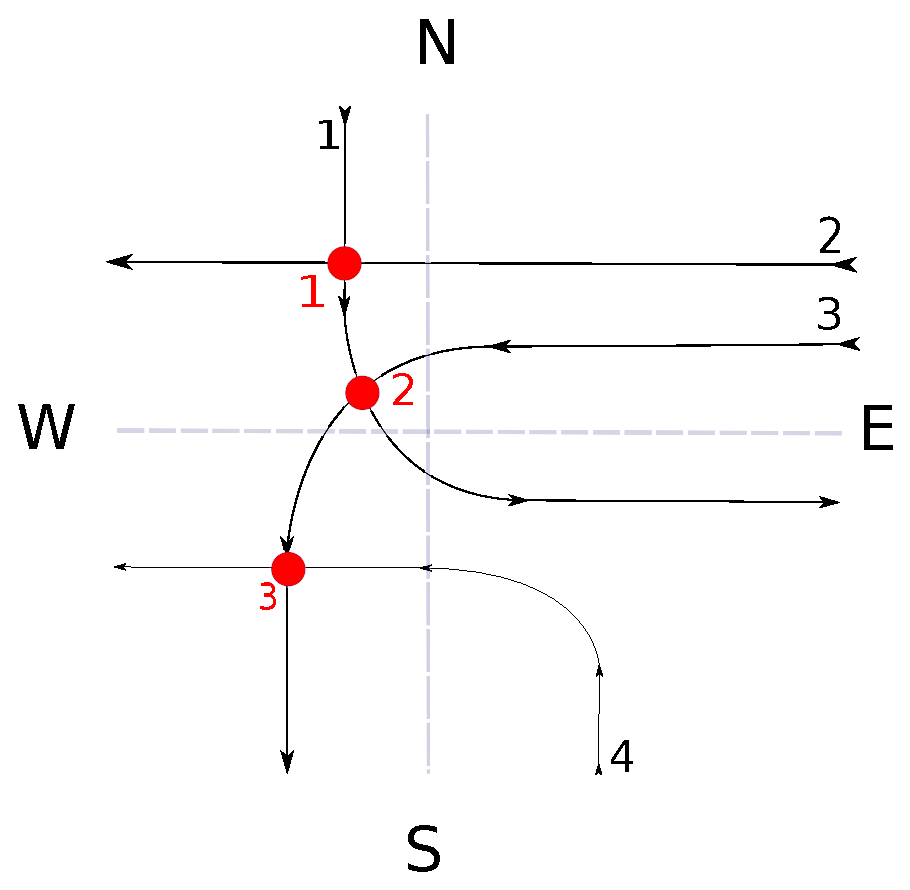
\includegraphics[width=\linewidth]{scheme.eps}
    \caption{Схема направлений и пересечерний для текущего варианта}
    \end{subfigure}
    \caption{Перекрёсток}
    \label{fig:1}
\end{figure}

\newpage

Каждое направление движения регулируется своим светофором. Если машин нет - светофор горит красным
светом. Если машины есть - светофор загорается зелёным (как только появится такая возможность)
и пропускает все машины, после чего снова загорается красным.
Требуется разработать модель контроллера светофоров, которая бы удовлетворяла следующим свойствам,
заданным в виде ltl формул.

Также в модели требуется отразить поведение внешней среды.

\lstinputlisting[language=Promela,numbers=left,%
firstline=1,firstnumber=1,lastline=38,%
caption={Формулы линейной темпоральной логики, отражающие требования к системе},%
label=ltl-formulae]{src/formulae.ltl}


\section{Построение модели}

\subsection{Внешняя среда}

Внешняя среда моделируется при помощи процессов, которые генерируют потоки машин по каждому
из доступных направлений. Каждый такой процесс посылает в бесконечном цикле сообщение о
прибывших машинах в канал ёмкостью 1, и затем блокируется до тех пор, пока это сообщение 
не будет обработано контроллером светофора, обслуживающего соответствующее направление 
движения.

\subsection{Дорожные пересечения}

Дорожные пересечения моделируются процессами, которые блокируются и разблокируются 
процессами светофоров.

\subsection{Светофоры}

Светофоры также моделируются соответствующими процессами. Суть работы светофора - при 
поступлении сообщения о наличии машин:

\begin{enumerate}
	\item Заблокировать соответствующие пересечения
	\item Пропустить поток машин
	\item Разблокировать "захваченные" пересечения в обратном порядке
\end{enumerate}

\subsection{Взаимодействие процессов}

Таким образом, модель состоит из процессов, моделирующих поведение светофоров, дорожных пересечений, а также из процессов, генерирующих потоки машин. Процесс, генерирующий поток машин для определённого направления, оставляет сообщение в канале $car\_sense[i]$ ёмкостью 1. Контроллер светофора, обслуживающий тоже направление, читает сообщение из этого канала, и затем начинает последовательно захватывать ресурсы (пересечения). Это делается посредством отправки сообщений процессам, обслуживающим соответствующие пересечения по каналам блокировки. Процесс, управляющий пересечением, читает сообщение о блокировке, отправляет
по рандеву каналу сообщение о подтверждении блокировки, и блокируется, ожидая сообщения 
об освобождении от блокирующего контроллера светофора. Когда контроллер светофора заблокировал все пересечения, через которые проходит регулируемый маршрут, 
он читает сообщение из канала о том, что машины ожидают проезда, меняет свой цвет на зелёный, и переключается обратно на красный. После этого отправляются сообщения о разблокировке пересечений в обратном порядке. Каналы, передающие пересечениям сообщения о блокировке, выглядят следующим образом:

\lstinputlisting[language=Promela,numbers=left,
firstline=23,firstnumber=23,lastline=25,
caption={Каналы сообщений, обеспечивающие взаимодействие процессов контроллеров светофоров и 
процессов дорожных пересечений},
label=channels]{src/model.pml}

Таким образом обеспечиватся последовательная обработка светофорами приходящие потоки машин по 
всем направлениям, а рандеву каналы позволяют осуществлять синхронное взаимодействие между 
процессами контроллеров светофоров и дорожных пересечений.

\section{Верификация алгоритма средствами spin}

При верификации, за один "такт" верификатор spin делает только 1 шаг в одном из активных процессов, тем
самым переводя систему в следующее состояние. Чтобы spin мог корректно верифицировать построенную модель,
будем проводить процедуру верификации при условии "слабой справедливости" \quad \cite{WeakFairness}. Эта опция spin
позволяет гарантировать, что каждый доступный к исполнению процесс рано или поздно будет
выбран верификатором spin для исполнения. Также при верификации были увеличены такие параметры, как доступный
 при верификации объём оперативной памяти, а также число допустимых
состояний, которое может быть достигнуто при верификации.

\section{Анализ результатов работы}

В результате работы были изучены особенности проектирования систем параллельных вычислений,
~\cite{verification} построена корректно работающая модель контроллера светофоров, а также получены практические
навыки работы с пакетом spin~\cite{spin}.

\pagebreak

\bibliographystyle{unsrt}
\bibliography{references}

\end{document}
